%% The following is a directive for TeXShop to indicate the main file
%%!TEX root = diss.tex

\chapter{True Positive Rates of Germline Variant Calling in FFPE Tumours}
\label{ch:TruePositiveRateofGermlineVariantCallinginFFPETumours}

Short recap of objectives \ldots

%%%%%%%%%%%%%%%%%%%%%%%%%%%%%%%%%%%%%%%%%%%%%%%%%%%%%%%%%%%%%%%%%%%%%
\section{Frequency of germline and somatic variants}
\label{sec:Frequencyofgermlineandsomaticvariants}
%%%%%%%%%%%%%%%%%%%%%%%%%%%%%%%%%%%%%%%%%%%%%%%%%%%%%%%%%%%%%%%%%%%%%

\begin{figure}[H]
\centering
	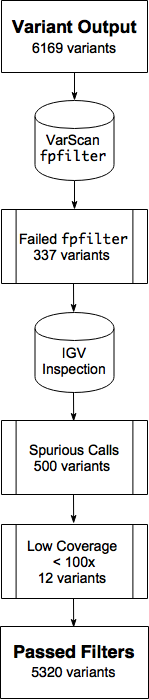
\includegraphics[scale=0.6]{variant_output.png}
	\caption{Add caption.}
	\label{fig:variant_output}
\end{figure}

%%%%%%%%%%%%%%%%%%%%%%%%%%%%%%%%%%%%%%%%%%%%%%%%%%%%%%%%%%%%%%%%%%%%%%
\section{Germline variants are highly concordant between blood and FFPE specimens}
\label{sec:GermlinevariantsarehighlyconcordantbetweenbloodandFFPEspecimens}

\begin{figure}[H]
\centering
	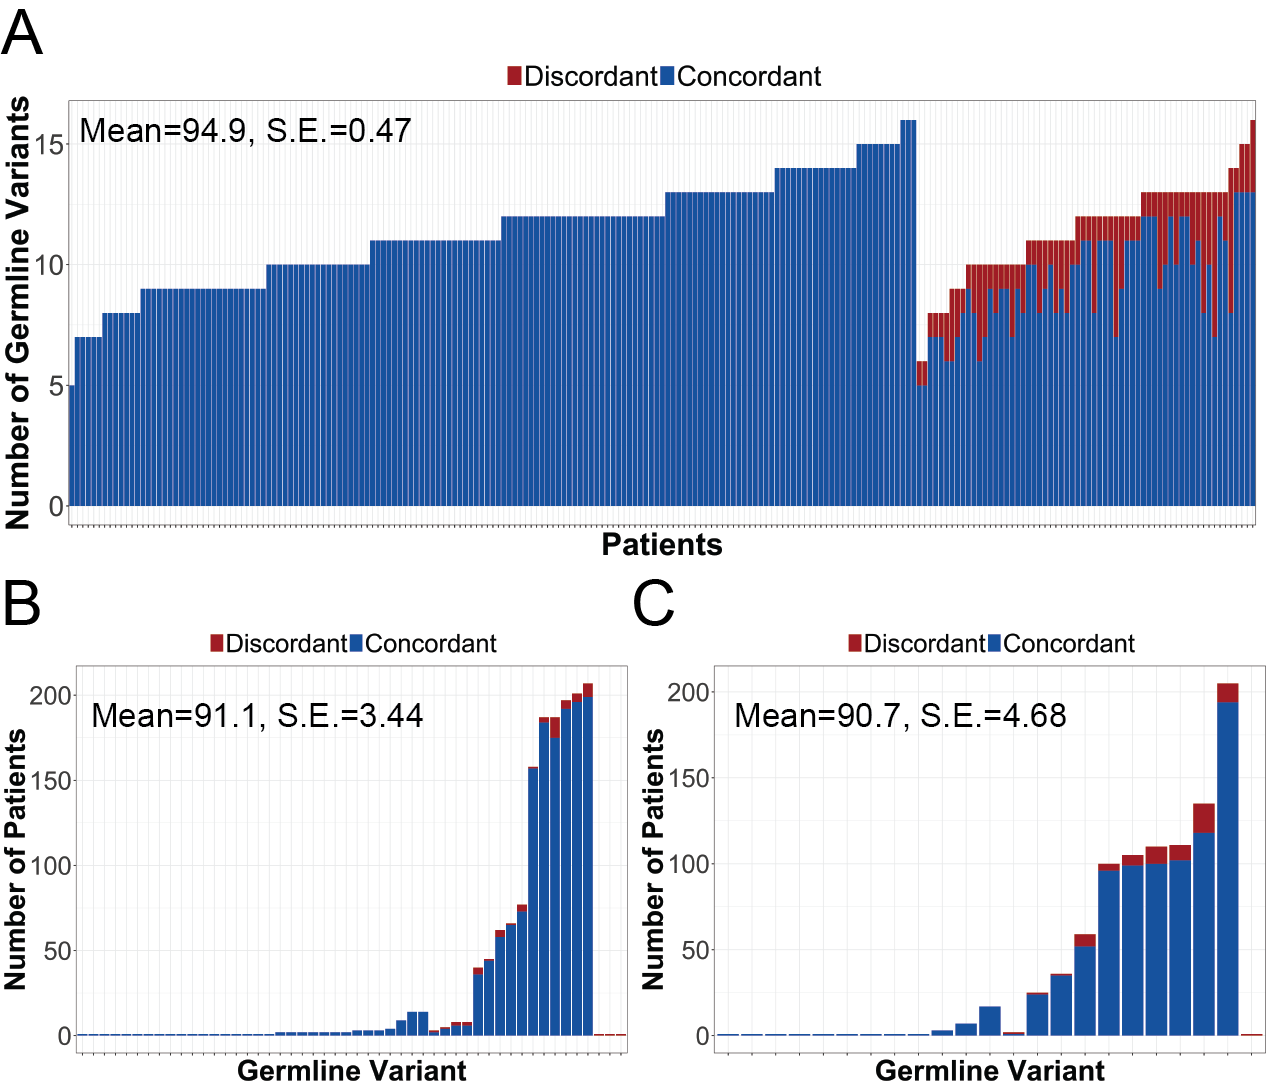
\includegraphics[scale=0.79]{true_positive_rate_variants.png}
	\caption{Add caption.}
	\label{fig:true_positive_rate_variants}
\end{figure}

%%%%%%%%%%%%%%%%%%%%%%%%%%%%%%%%%%%%%%%%%%%%%%%%%%%%%%%%%%%%%%%%%%%%%%
\section{Reduced sensitivity is observed for detection of germline variants in FFPE specimens compared to blood}
\label{sec:ReducedsensitivityisobservedfordetectionofgermlinevariantsinFFPEspecimenscomparedtoblood}

\begin{figure}[H]
	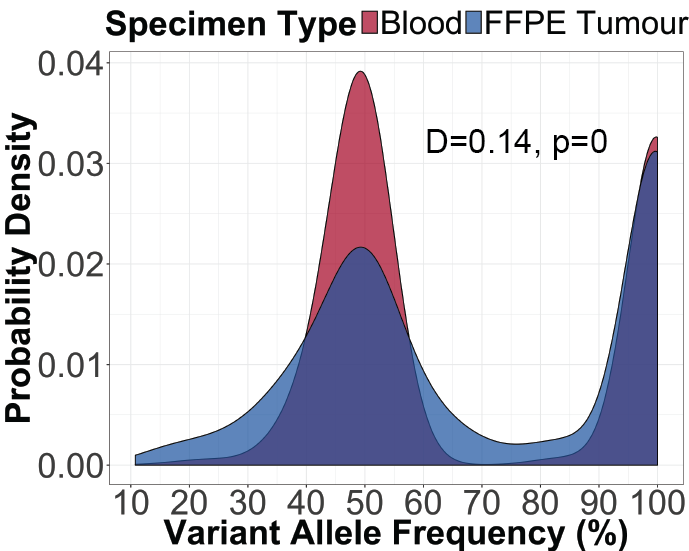
\includegraphics[scale=0.7]{germline_vaf_sens.png}
	\caption{Add caption.}
	\label{fig:germline_vaf_sens}
\end{figure}

\begin{table}[H]
\caption{Sensitivity of detecting germline variants in blood and FFPE specimens at various variant allele frequency thresholds.}
\label{sensitivity}
\centering
      \begin{tabular}{cllcclllccl}
        \hline
				\multicolumn{1}{l}{ }
				&
				\multicolumn{4}{l}{Blood}
				&&
				\multicolumn{4}{l}{FFPE Tumour}
        \\
				\cline{2-5}\cline{7-10}
        VAF (\%) & FN\mbox{*} & TP\mbox{**} & Sensitivity & 95\% CI && FN\mbox{*} & TP\mbox{**} & Sensitivity & 95\% CI
        \\
        \hline
        10 & 0 & 2461 & 1.0 & 1.0--1.0 && 0 & 2428 & 1.0 & 1.0--1.0
        \\
        15 & 2 & 2459 & 1.0 & 1.0-1.0 && 12 & 2416 & 1.0 & 0.99--1.0
        \\
        20 & 3 & 2458 & 1.0 & 1.0--1.0 && 48 & 2380 & 0.98 & 0.97--0.99
        \\
        25 & 15 & 2446 & 0.99 & 0.99--1.00 && 79 & 2349 & 0.97 & 0.96--0.97
        \\
        30 & 20 & 2441 & 0.99 & 0.99--1.00 && 121 & 2307 & 0.95 & 0.94--0.96
        \\
        35 & 33 & 2428 & 0.99 & 0.98--0.99 && 197 & 2231 & 0.92 & 0.91--0.93
        \\
        40 & 107 & 2354 & 0.96 & 0.95--0.96 && 328 & 2100 & 0.86 & 0.85--0.88
        \\
        45 & 234 & 2227 & 0.90 & 0.89--0.92 && 470 & 1958 & 0.81 & 0.79--0.82
        \\
				\hline
      \end{tabular} \\
\end{table}

\begin{figure}[H]
	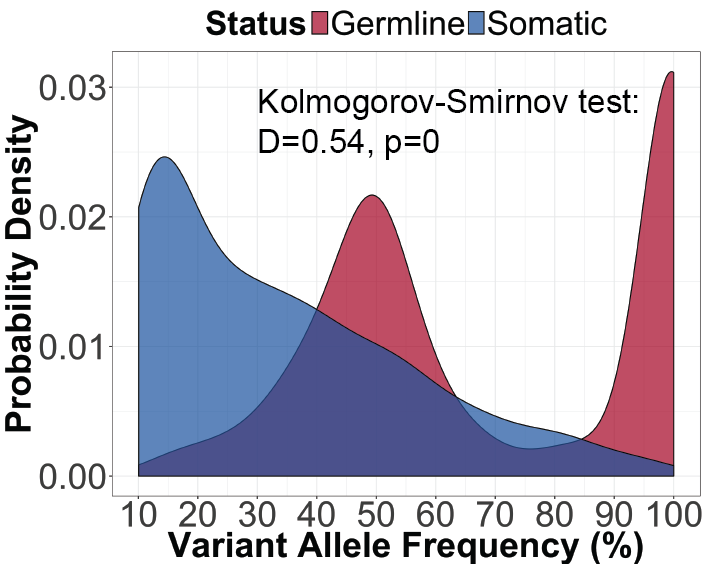
\includegraphics[scale=0.7]{germline_somatic_ppv.png}
	\caption{Add caption.}
	\label{fig:germline_somatic_ppv}
\end{figure}

\begin{table}[H]
\caption{Positive predictive value for referral of potential germline variants for downstream confirmatory testing.}
\label{ppv}
\centering
      \begin{tabular}{ccccccl}
        \hline
        VAF (\%) & False Positive & True Positive & Total Calls & Positive Predictive Value & 95\% CI
        \\
        \hline
        10 & 431 & 2428 & 2859 & 0.85 & 0.84--0.86
        \\
        15 & 319 & 2416 & 2735 & 0.88 & 0.87--0.90
        \\
        20 & 273 & 2380 & 2653 & 0.90 & 0.88--0.91
        \\
        25 & 245 & 2349 & 2594 & 0.91 & 0.89--0.92
        \\
        30 & 203 & 2307 & 2510 & 0.92 & 0.91--0.93
        \\
        35 & 178 & 2231 & 2409 & 0.93 & 0.91--0.94
        \\
        40 & 146 & 2100 & 2246 & 0.93 & 0.92--0.94
        \\
        45 & 118 & 1958 & 2076 & 0.94 & 0.93--0.95
        \\
				\hline
      \end{tabular} \\
\end{table}


%%%%%%%%%%%%%%%%%%%%%%%%%%%%%%%%%%%%%%%%%%%%%%%%%%%%%%%%%%%%%%%%%%%%%%
\section{Factors underlying reduced sensitivity of germline variant calling in FFPE specimens}
\label{sec:FactorsunderlyingreducedsensitivityofgermlinevariantcallinginFFPEspecimens}

%%%%%%%%%%%%%%%%%%%%%%%%%%%%%%%%%%%%%%%%%%%%%%%%%%%%%%%%%%%%%%%%%%%%%
\section{Discussion}
\label{sec:Discussion}
%%%%%%%%%%%%%%%%%%%%%%%%%%%%%%%%%%%%%%%%%%%%%%%%%%%%%%%%%%%%%%%%%%%%%

\endinput
\pagebreak
\begin{table}[H]
\caption{Frequency of germline and somatic variants detected in the tumours of 213 patients in the TOP cohort.}\label{freqvariants}
\centering
\begin{tabular}{lcclcl}
        \hline
        Gene & Germline & Pathogenic Germline && Somatic \\
				 & (N Patients) & (N Patients) && (N Patients) \\
				\hline
				\\
				\multicolumn{1}{l}{\textit{Cancer predisposing}}
				&
				\multicolumn{2}{l}{ }
				&&
				\multicolumn{1}{l}{} \\
				\hline
				AKT1 & 0 & 0 && 2 (2) \\
				\arrayrulecolor{evagrey}\hline
				ALK & 1 (1) & 1 (1) && 2 (1) \\
				\hline
				BRAF & 0 & 0 && 18 (17) \\
				\hline
				EGFR & 170 (164) & 5 (5) && 31 (24) \\
				\hline
				HRAS & 0 & 0 && 1 (1) \\
				\hline
				MAP2K1 & 0 & 0 && 2 (2) \\
				\hline
				MAPK1 & 17 (17) & 3 (3) && 3 (2) \\
				\hline
				MTOR & 763 (213) & 6 (6) && 71 (30) \\
				\hline
				NRAS & 0 & 0 && 8 (8) \\
				\hline
				PDGFRA & 242 (185) & 0 && 8 (4) \\
				\hline
				PIK3CA & 0 & 0 && 15 (4) \\
				\hline
				PTEN & 0 & 0 && 1 (1) \\
				\hline
				STAT1 & 54 (51) & 1 (1) && 7 (6) \\
				\hline
				STAT3 & 10 (10) & 4 (4) && 16 (11) \\
				\hline
				TP53 & 189 (184) & 2 (2) && 131 (109) \\
				\arrayrulecolor{black}\hline
				\\
				\multicolumn{1}{l}{\textit{Pharmacogenomics}}
				&
				\multicolumn{2}{l}{ }
				&&
				\multicolumn{1}{l}{} \\
				\arrayrulecolor{black}\hline
				DPYD & 271 (212) & 1 (1) && 1 (1) \\
				\arrayrulecolor{evagrey}\hline
				GSTP1 & 106 (106) & 0 && 0 \\
				\hline
				MTHFR & 209 (177) & 0 && 0 \\
				\hline
				TYMP & 81 (76) & 2 (2) && 18 (13)\\
				\hline
				TYMS & 131 (131) & 0 && 0 \\
				\hline
				UGT1A1 & 96 (96) & 0 && 1 (1) \\
				\arrayrulecolor{black}\hline \\
				Total & 2396 (213*) & 25 (23*) && 431 (180*) \\
				\arrayrulecolor{black}\hline
      \end{tabular}
\end{table}
